\documentclass[review]{elsarticle}


\usepackage{amsmath,lineno,amsthm,verbatim,graphicx}
\usepackage{hyperref}
\modulolinenumbers[5]

\journal{Economic Letters}


%%%%%%%%%%%%%%%%%%%%%%%
%% Elsevier bibliography styles
%%%%%%%%%%%%%%%%%%%%%%%
%% To change the style, put a % in front of the second line of the current style and
%% remove the % from the second line of the style you would like to use.
%%%%%%%%%%%%%%%%%%%%%%%

%% Numbered
%\bibliographystyle{model1-num-names}

%% Numbered without titles
%\bibliographystyle{model1a-num-names}

%% Harvard
%\bibliographystyle{model2-names.bst}\biboptions{authoryear}

%% Vancouver numbered
%\usepackage{numcompress}\bibliographystyle{model3-num-names}

%% Vancouver name/year
%\usepackage{numcompress}\bibliographystyle{model4-names}\biboptions{authoryear}

%% APA style
%\bibliographystyle{model5-names}\biboptions{authoryear}

%% AMA style
%\usepackage{numcompress}\bibliographystyle{model6-num-names}

%% `Elsevier LaTeX' style
\bibliographystyle{elsarticle-num}
%%%%%%%%%%%%%%%%%%%%%%%
\newtheorem{thm}{Theorem}
\newtheorem{lemma}{Lemma}
\newtheorem{prop}{Proposition}

\begin{document}

\begin{frontmatter}

\title{ Reserve Price vs Experience Fee in Auction for Experience Good}


%% Group authors per affiliation:
\author{Yan Ju\corref{mycorrespondingauthor}, Dazhong Wang\fnref{myfootnote}}
\address{Wuchuan Road 111, Shanghai }
\address[mymainaddress]{School of Economics}
\address[mysecondaryaddress]{Shanghai University of Finance and Economics}
\fntext[myfootnote]{Both are PhD students from SOE.}
\cortext[mycorrespondingauthor]{Corresponding author's email address}
\ead{juyan255@126.com, wangdazhongab@163.com}


\begin{abstract}
This paper discusses revenue maximization for the seller of an indivisible
good under an auction situation when bidders all have the same
value distribution of the given auction good ex ante. In the paper's
setting, seller can give buyer access to get his true value without
cost, which we call "experience" of the good.If the seller is
unable to charge, she can increase her revenue by  letting a certain subset of  bidders experience the good. What's interesting is 
that  under many distributions, it is better for the seller to exclude just one bidder from experiencing, which is in conflict with the social efficiency. If
the seller is able to charge for the experience, she will maximize her revenue  through setting
the price at a level such that every potential buyer will buy the experience,
which results in the maximal trading surplus.
\end{abstract}

\begin{keyword}
 auction, experience good, reserve price, experience fee
\end{keyword}

\end{frontmatter}



\section{Introduction}
Regretting buying a new good after winning a bidding is
generally more common than regretting without winning the bidding. In
private value auction setting, there is such phenomenon. The
explanation for that is the buyers' value uncertainty. There are
recently many literature trying to solve such a problem of buyers'
value uncertainty.

 Quoting Riley  and  Samuelson(1981)\cite{Samuelson81} ,  "the
choice  of  auction  method  employed  rests  with the  monopolistic
seller ". Cremer(1988)\cite{Jacques88} has characterized
auctions  for  a single  indivisible  object  in the  case  where  the
bidders  have information  about  each  other  which  is not available  to the  seller, and the seller can get full  extraction  of  the  surplus  in bayesian  and
dominant  strategy  auctions. Myerson(1981)\cite{Myerson81} discussed
optimal auction design in the private value indivisible good
case. For instance,  Zhang(2013)\cite{Jun13} has taken
return policy into examination for solving buyers' value uncertainty
ex ante.  Cremer(2009)\cite{Jacques09} tries to consider
costly information acquisition's effect on auctions in buyers' value
uncertainty settings. Bergeman and pesendorfer(2007)\cite{Bergemann07}
has considered Information structures in optimal auctions when the
seller has full control over the information precision that the
bidders can get under costless revelation. They analyze the best
information structure for the seller under the  assumption that the seller
can give out signals that are arbitrarily correlated to the true value
of each buyer and the signal is free.What distinguish our work from Bergeman(2007)\cite{Bergemann07} setup is
 that if the experience is seen as a signal the
seller can only choose two extremes,no signal or the true
value signal itself, instead of arbitrary precision signals. And we consider the possibility of selling the experience(true value signal).
This is a big difference from Bergemann\cite{Bergemann07}'s paper. They have not considered the case of charging fee. Their focus is on the information structure decision 
by the seller given this choice. Here we model the pricing behavior when the seller only has the choice between revealing the true value or leave it alone.

This paper investigates risk-neutral rational individual's behaviors in an auction where the good for auction has the same value distribution ex ante to all bidders. Assuming the same prior for all the buyers involved is not unpractical when the good is a new product or something no buyer have experienced before.
Therefore this paper adopts such a rather simple same prior setting in order to get some intuition to penetrate the cloud of inherent complexity associated with uncertainty.Also we assume no friction of information revelation, that is , the cost of the seller revealing to a buyer his true value of the auction good and the gain of the buyer by just enjoying the revelation process are both zero. 
This assumption makes the seller control the information revelation more freely(though he does not know the private value of the good for any bidder even after the revelation!).
If the seller is unable to charge fee, he may discriminate one buyer by not letting him to get the experience, in order to have a option of selling the good to him at $\mu$. If the seller is able to charge fee for experiencing the good, then the seller
will set a price of experience acceptable to all buyers , thus results in social efficiency, but all the surplus is extracted by the seller.

The rest of the paper is organized as follows. Section 2 describes
the model. Section 3 characterizes a revenue-maximizing seller's
strategy when he is unable to sell the information, and the social efficiency
loss and discrimination behavior which may happen in this
situation. Section 4 gives a Revenue maximizing solution when the seller can sell the true value signal. Section 5 is the conclusion of the model.

\section{Model setup}

A seller(she) has a single indivisible good, and
designs a mechanism to sell the good to a group of $n$ buyers indexed by $i=1,2,...,n$(buyers and
bidders are used interchangeably in this paper, and are assumed to be
male). All parties are risk neutral.
 The reservation value of the seller
is publicly known, which is the value the seller gets
if she retains the object. It is normalized to $\underline{v}(\geq 0)$ in this paper.Bidder i's valuation of the object
is $v_{i}$, and $v_{i}$ has independent identical distribution $F(x)$ with support $[\underline{v},\overline{v}]$,
where $\overline{v}>\underline{v}$, and $\overline{v}=+\infty$ is allowed. 
In the beginning, no one can directly observe the $v_{i}$ and the distribution is common knowledge. However, if the seller gives a chance of experiencing the good to a buyer, the buyer can learn of his $v_{i}$ after experiencing.
 

The seller would like to use a common auction form to sell the
good.  The sales mechanism consists of two stages, the experience-stage, and the auction-stage. By  Revenue Equivalence Principle, we choose the second-price
sealed bid auction in the auction-stage without loss of generality.
After the  experience-stage, the seller will allow those who
have experienced the good(received the true value signal) to
participate the auction. If no bidder bids a value exceeding the
reserve price, then the good is sold to the unexperienced buyers with the
price $\mu$, the expectation of v, and as a risk neutral buyer he will buy it.







\section{Setting Reserve price to extract trade surplus}
In the situation that the seller cannot charge fee for the information
revelation,  the seller can set a reserve price in the bidding stage to maximize the
revenue in a second-price sealed-bid auction. The corresponding
optimal reserve price $r$ satisfies $r - \frac{1 - F(r)}{f(r)}
= v^*$, independent of the number of buyers getting experience
opportunity. The $v^*$ denotes the seller's reserve valuation/revenue. 
 The number of buyers who can get the true value signal is at her control. If she gives the true
signal, no one will refuse since getting the signal means some chance
of gain. Intuitively, she 
wants more buyers to know their true value in order to have a high
revenue in the bidding as long as there is still a potential buyer who
has not bought the experience and the seller can sell the good to him
at price $\mu$ in the event of no bidders having bidden over the
reserve price. This is summarized in the following proposition.
\begin{prop}
 As the number m of buyers knowing one's own value information increases, the expected value of seller revenue increases as long as $m<n-1$.
\end{prop}
\begin{proof}
When there are m$(m\leq n-1)$ buyers knowing one's own value information, the expected value of seller revenue can be calculated.
If the seller decides to have $m$ buyers to experience and set the
reserve price at $r^*$, which is the solution to $r^*-\frac{1 - F(r^*)}{f(r^*)}=\mu$. We have
\begin{equation}
R(r^* ;m) =  \int_{r^*}^{\overline{v}}x\mathrm{d}G_{(2)}^{m}(x) +
r^*(m)F^{m-1}(r^*)[1 - F(r^*)] + \mu F^{m}(r^*)
\end{equation}
where $G_{(2)}^{m}(x) = F^{m}(x) + (m)F^{m-1}(x)[1 -  F(x)]$.
 By the first order stochastic dominance, it is straightforward to show $R(r^*;m) > R(r^*;m')$ for any $n>m>m'$.
\end{proof}
However, lettingNpotential buyers to all know their true value may
not be better than just letting n-1 buyers. Because this may let go the
safe option of selling the good at $\mu$. Indeed, it depends on the
distribution F(x). A careful research of us has led to the following conclusion.
\begin{thm}
  The seller does not always want all buyers to know the true value. 
 When every buyers know their value, 
 the reserve price should now be set to $\hat{r}$, which is the solution to $\hat{r}-\frac{1 - F(\hat{r})}{f(\hat{r})}=0$, and the revenue is $R(\hat{r},n)$ using formula (1). Compared to the $R(r^*,n-1)$,
 $R(\hat{r},n)<R(r^*,n-1)$ for many distributions and the potential buyers' number n.
 \end{thm}

The  graph shows the value of $R(N-1)-R(N)$ for some
values of parameters in Beta distribution.
(with the blue line being the uniform distribution, and the other 5 being beta distribution with a=1, and b= 5, 10, 15, 20, 25.).
\begin{figure}
\centering
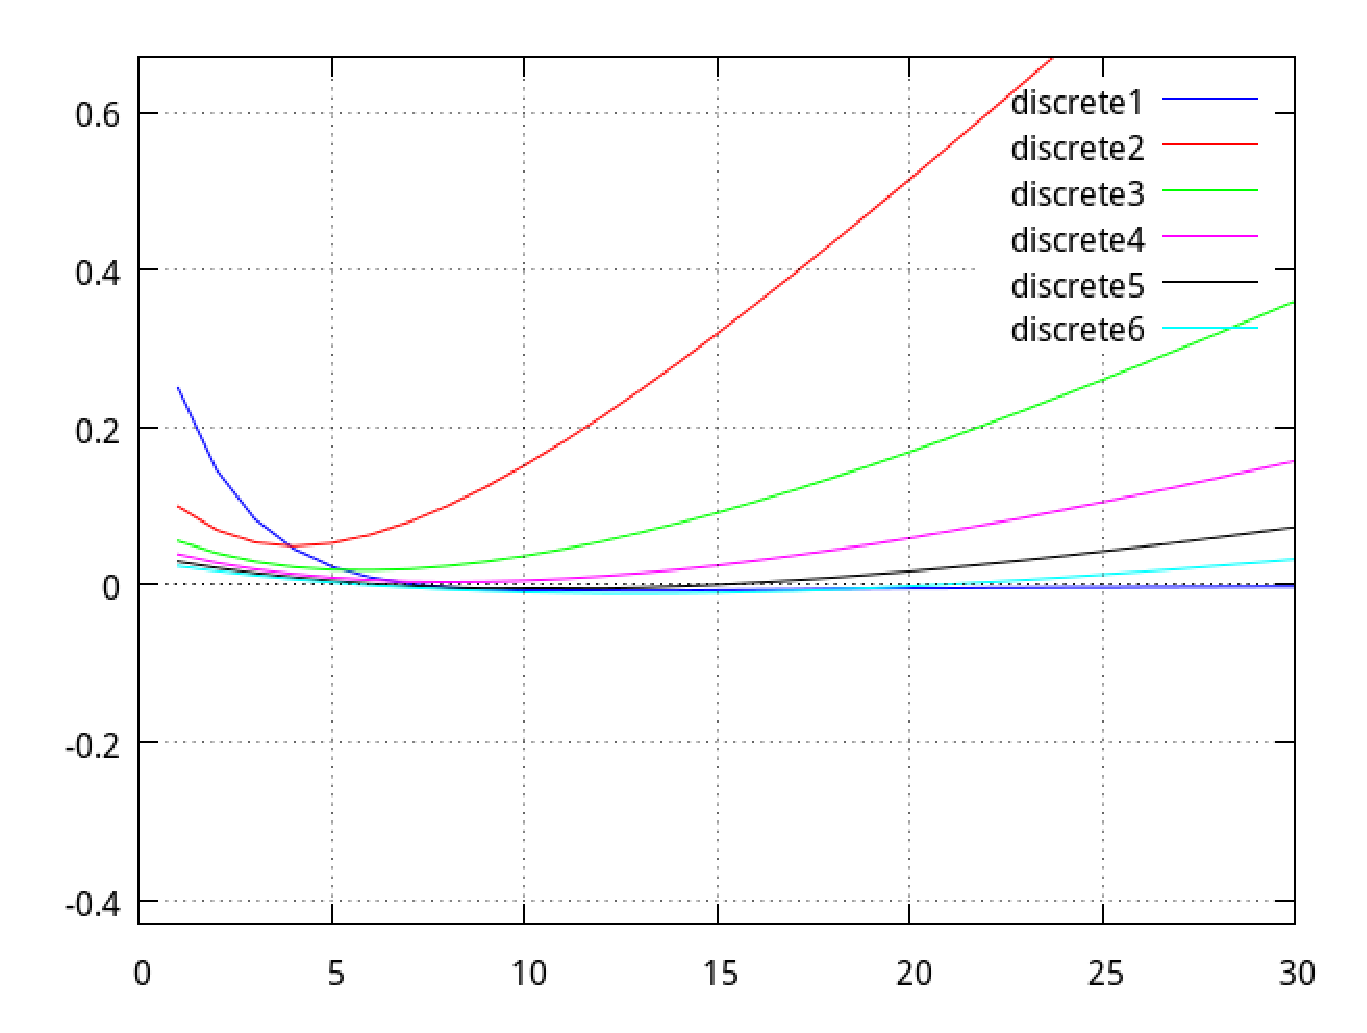
\includegraphics[width = 7cm]{mypic.eps}
\caption{Difference in revenue} \label{fig:graph}
\end{figure}
Specially for the uniform distribution, when $n\leq 7$, $R(\hat{r},n)<R(r^*,n-1)$.
\section{Charging Experience fee to extract trade surplus}
  We then consider the case where the seller can charge experience fee. For the seller, at the experience-stage, how to optimally set price of exprience?
If a certain number of buyers are permitted to experience the good, each of those buyers is supposed to  get a nonnegative ex ante expected payoff from participating the
subsequent second-price auction.  Suppose that buyers will buy the experience when they are indifferent between remaining
uninformed and buying the experience to be informed.
 Then the seller should set the price equal to a buyer's ex ante expected payoff of participating the auction to extract all the expected trade surplus.
 Interestingly, the ex ante expected payoff of experiencing buyers  depends on the number of auction partipants.

Next, we will offer the formula for the experience fee in the following lemma.
\begin{lemma}
  The experience fee $P(m)$ can be formulated as 
  \begin{align}
 P(m)
= \begin{cases}\int_{\mu}^{\overline{v}}\int_{\mu}^vF^{m-1}(t)\mathrm{d}tf(v)\mathrm{d}v, & \textrm{if $m \leqN-1$}\\
\int_{\underline{v}}^{\overline{v}}\int_{\underline{v}}^v F^{n-1}(t)\mathrm{d}tf(v)\mathrm{d}v, &\textrm{if $m = N$}\\
\end{cases}
\end{align}
\end{lemma}
\begin{proof}
  When there are $m(\leq n-1)$ buyers knowing one's own value information, the value of the information is
\begin{align*}
P(m)&= \int_{\mu}^{\overline{v}}(\int_{\mu}^v (v-t)\mathrm{d}F^{m-1}(t)+(v-\mu)F^{m-1}(\mu))f(v)\mathrm{d}v\\
&= \int_{\mu}^{\overline{v}}\int_{\mu}^vF^{m-1}(t)\mathrm{d}tf(v)\mathrm{d}v
\end{align*}

$P(N)$ can be formulated as,

  \begin{align*}
P(N) &= \int_{\underline{v}}^{\overline{v}}\int_{\underline{v}}^v(v-t)\mathrm{d}F^{n-1}(t)\mathrm{d}tf(v)\mathrm{d}v \\
 &= \int_{\underline{v}}^{\overline{v}}\int_{\underline{v}}^v F^{n-1}(t)\mathrm{d}tf(v)\mathrm{d}v
  \end{align*}
\end{proof}

\begin{lemma}
As the number of buyers knowing one's own value information increases, the expected value of knowing one's own value information decreases.
\end{lemma}
Notice that for many distributions and potential buyers' number n,  $P(N) < P(N-1)$. In such cases, the seller set price at $P(N)$, and 
the buyers' domininant stratey is to buy the experience.
Since every buyer knows the true value in the auction and expected gain of every buyer is zero now, the seller can extract full surplus through setting appropriate experience fee.  the 
social surplus is maximized and fully extracted by the seller.



The above reasoning leads to the following conclusion

\begin{thm}

 If the seller can charge fee for letting one buyer know his true value, then the seller will set the price at
 $ \int_{\underline{v}}^{\overline{v}}\int_{\underline{v}}^v F^{n-1}(t)\mathrm{d}tf(v)\mathrm{d}v$ to  fully extract all the surplus of trade, and the revenue she get is 
 \begin{equation}
  E(v_{(1)}^n)=\int_{\underline{v}}^{\overline{v}} x\mathrm{d}F^n(x) 
 \end{equation}
\end{thm}
 This is the best possible result for the seller, maximizing the trade surplus and minimizing all the buyers' share.






\section{Conclusion}

The paper is supposed to shed light on a seller's optimal
sales mechamism design when buyers have identical  value distribution about the
experience good, but do not know the private value before the experience. The seller controls the number of buyers to experience.

When the seller is not able to charge experience fee, her optimal sales mechanism might be to exclude a buyer from experiencing the good, which harms social
 efficiency. When the seller is allowed to charge fee, the result is efficient. However, the defect is that
 all the trade surplus is extracted  by the seller.
 
\begin{comment}
\section{Bibliography styles}

There are various bibliography styles available. You can select the style of your choice in the preamble of this document. These styles are Elsevier styles based on standard styles like Harvard and Vancouver. Please use Bib\TeX\ to generate your bibliography and include DOIs whenever available.

Here are two sample references: \cite{Feynman1963118,Dirac1953888}.
\end{comment}

\section*{References}

\bibliography{RevenueMax}

\end{document}
